\documentclass{article}
\usepackage{graphicx}
\usepackage{amsmath}
\usepackage{booktabs}
\usepackage{geometry}
\usepackage{microtype}
\usepackage[colorlinks=true,linkcolor=blue,citecolor=blue,urlcolor=blue]{hyperref}
\usepackage{orcidlink}
\usepackage{silence}
\WarningFilter{latex}{Command \showhyphens has changed}
\geometry{left=2.5cm,right=2.5cm,top=2.5cm,bottom=2.5cm}


\title{Replacing Dark Energy and Unifying Large-Scale Anomalies: \\ The Progenitor Node Model within a Virialized Meta-Structure}
\author{Martin Gamsby\,\orcidlink{0009-0007-4069-9687}}
\date{May 2026}

\begin{document}

\maketitle

\begin{abstract}
Standard $\Lambda$CDM cosmology \cite{Planck2020} attributes late-time cosmic acceleration to dark energy: a vacuum energy term that fits observations but has no physical explanation.
It requires a 120-order-of-magnitude fine-tuning of vacuum energy \cite{Weinberg1989} and an unexplained coincidence between matter and dark energy densities \cite{Steinhardt1999}.

We present a toy model, the \textbf{External-Node Model}, in which the observable universe is a finite Friedmann-Robertson-Walker (FRW) region expanding within a lattice of Hyper-Massive External Attractors (HMEAs).
In this model, cosmic acceleration comes from tidal gravity. As the bubble expands toward neighboring nodes, it is pulled apart. No exotic physics required.

N-body simulations over the late-universe era ($t=5.8 \rightarrow 13.8$ Gyr) reproduce $\Lambda$CDM expansion with \textbf{$R^2 > 0.95$ for expansion rate} and \textbf{$R^2 > 0.99$ for size}, using configurations spanning $M = 92$-$9000 \times M_{obs}$, $S = 15$-$38$ Gpc.

The same lattice geometry, with no additional parameters, also produces patterns consistent with three large-scale anomalies: the Hubble Tension ($\Delta H_0/H_0 \approx 5$-$11\%$ \cite{Riess2022}), the CMB ``Axis of Evil'' \cite{Land2005}, and dark flow \cite{Watkins2023}. We do not attempt to model early-universe dynamics or provide a complete theoretical resolution to these large-scale anomalies; rather, our simulation provides a proof-of-concept that classical gravity is sufficient to reproduce late-time acceleration, implying that tidal forces alone might account for the dynamics we currently label as dark energy.
\end{abstract}

\section{Introduction}
\label{sec:intro}

The accelerating expansion of the universe \cite{Riess1998, Perlmutter1999} is conventionally explained by a constant vacuum energy density: the Cosmological Constant ($\Lambda$).
$\Lambda$CDM fits the data well ($\Omega_\Lambda \approx 0.7$), but has two serious problems.

The \textbf{Fine-Tuning Problem} \cite{Weinberg1989}: quantum field theory predicts a vacuum energy 120 orders of magnitude larger than observed.
Matching observation requires cancellation to extraordinary precision.

The \textbf{Coincidence Problem} \cite{Steinhardt1999}: dark energy and matter densities happen to be comparable ($\Omega_\Lambda \sim \Omega_m$) in the present epoch. This is a statistically unlikely coincidence with no explanation.

\textbf{We propose a different interpretation.} Rather than assuming the FRW metric describes all of spacetime, we model the observable universe as a finite FRW region expanding within a larger space containing discrete massive objects.
In this picture, ``dark energy'' is a misidentification: the \textbf{intrinsic repulsion} attributed to the vacuum is actually \textbf{extrinsic attraction} from a surrounding mass distribution.
We call this the \textbf{External-Node Model}.
This resolves the fine-tuning problem directly: gravity is weak at large scales, so the required forces are small.
A companion \textbf{Progenitor Hypothesis} (Section~\ref{sec:progenitor}) addresses isotropy. In this hypothesis, the Big Bang would have originated from a destabilized node within the meta-structure, inheriting the symmetry of its equilibrium position.

The idea that trans-observable structure could affect cosmological dynamics is not new.
Mersini-Houghton and Holman \cite{MersiniHoughton2009} proposed that entanglement with neighboring landscape domains could produce bulk flows and CMB anomalies; others have noted that matter beyond the particle horizon could source coherent motions \cite{Kashlinsky2008}.
But prior proposals address individual anomalies with purpose-built mechanisms.
Our framework is different: a single lattice geometry, motivated by the need to reproduce cosmic acceleration, naturally yields patterns consistent with the Hubble Tension, the CMB ``Axis of Evil,'' and dark flow (Section~\ref{sec:predictions}) as an immediate consequence, with no additional parameters. This unification under one geometric structure is, to our knowledge, novel.

\section{The Physical Model}
\label{sec:model}

\subsection{The Virialized Grid Topology}
\label{sec:grid}
Standard cosmology assumes the Cosmological Principle (homogeneity and isotropy) holds at all scales.
We propose that it holds only within our local bubble.
Beyond our horizon, we model a \textbf{Virialized Meta-Structure}: a gravitationally balanced arrangement of mass concentrations, stable over vast timescales but irregular in detail—much like galaxies within a relaxed cluster.

These concentrations, termed \textbf{Hyper-Massive External Attractors (HMEAs)}, are compact objects far older than 13.8 Gyr, with masses $M_{ext} \gg M_{obs}$, separated by voids much larger than the observable universe.
Our universe sits in one such void, expanding toward the surrounding nodes.


\subsection{The Progenitor Hypothesis}
\label{sec:progenitor}
A standard objection to bubble cosmologies: why is our universe at the center of the void, making expansion appear isotropic?

The \textbf{Progenitor Hypothesis} answers this.
The Big Bang was not a creation event \textit{ex nihilo} in random empty space, but the destabilization of a specific object:

\begin{enumerate}
\item \textbf{Origin}: Our universe originates from a \textbf{Progenitor Node} located at the gravitational equilibrium point between its neighbors, which was formerly a member of the Virialized Grid.
\item \textbf{Event}: The Progenitor Node destabilized (via critical mass accumulation, quantum instability, or collision) and transitioned from a stable object into a rapidly expanding cloud of matter and radiation.
\item \textbf{Isotropy}: Because the Progenitor Node was positioned at the equilibrium point, its subsequent expansion proceeded symmetrically into the potential wells of the surrounding structure, naturally accounting for isotropy without fine-tuning.
\end{enumerate}

\section{Dynamics and Quantitative Analysis}
\label{sec:dynamics}
Expansion is governed by two competing forces: internal self-gravity (deceleration) and external tidal gravity (acceleration), with the latter acting as the physical mechanism replacing dark energy.

\subsection{The Tidal Acceleration Mechanism}
\label{sec:tidal}
Under the standard shell theorem, a continuous spherical external distribution exerts no net force, meaning deceleration is governed entirely by the enclosed mass $M_{int}$. Our lattice geometry alters this dynamic: because the external mass is concentrated in discrete nodes rather than a smooth shell, it generates a net tidal pull.

To model this effect in three dimensions using the simplest possible symmetric geometry, we arrange the external mass concentrations into a $3\times3\times3$ lattice containing 26 nodes. While the real-world distribution would be far more irregular, this idealized lattice allows us to isolate the core physics. At the exact center of this grid ($R=0$), the forces from the surrounding nodes perfectly cancel. However, as our expanding universe moves outward, it climbs the potential gradient of the nearest HMEA, and the resulting tidal force increases with distance from the center.

Evaluating this tidal contribution along a single axis toward the nearest node, the acceleration from an external mass $M_{ext}$ at a grid distance $S$ is given by:

\begin{equation}
a_{tidal} \approx \frac{G M_{ext}}{(S - R)^2} - \frac{G M_{ext}}{S^2}
\label{eq:tidal-exact}
\end{equation}

For $R \ll S$, Taylor expansion gives a linear dependence on $R$:

\begin{equation}
a_{tidal} \approx \frac{2 G M_{ext}}{S^3} R
\label{eq:tidal-linear}
\end{equation}

While this single-axis derivation isolates the nearest node, it captures the correct linear-in-$R$ scaling and provides a sound order-of-magnitude estimate of the tidal field. At the central equilibrium point ($R = 0$), all forces cancel. As the universe expands, tidal forces scale as $\sim G M / d^3$, so the nearest face node at distance $S$ dominates over edge nodes at $S\sqrt{2}$ ($\sim 35\%$ contribution) and corner nodes at $S\sqrt{3}$ ($\sim 19\%$). The full 26-node system is accounted for in our numerical simulation (Section~\ref{sec:numerical}).

The critical result here is the linear $R$ dependence. In the standard Friedmann equations, the cosmological constant drives an acceleration of $H_0^2 \Omega_\Lambda R$. Consequently, in the non-relativistic limit, this uniform external tidal field is mathematically indistinguishable from $\Lambda$.

\subsection{Estimation of Required Node Mass and Distance}
\label{sec:estimation}
Equating the tidal acceleration (Equation~\ref{eq:tidal-linear}) to the observed dark energy acceleration:

\begin{equation}
H_0^2 \Omega_\Lambda \approx \frac{2 G M_{ext}}{S^3}
\label{eq:matching}
\end{equation}

Solving for the grid spacing $S$:

\begin{equation}
S \approx \left( \frac{2 G M_{ext}}{H_0^2 \Omega_\Lambda} \right)^{1/3}
\end{equation}

Assuming $M_{ext} = 5 \times 10^{55} \text{ kg}$ ($\approx 500 \times M_{obs}$, where $M_{obs} \approx 10^{53} \text{ kg}$), $H_0 \approx 70 \text{ km/s/Mpc} \approx 2.3 \times 10^{-18} \text{ s}^{-1}$, and $\Omega_\Lambda \approx 0.7$:

\begin{equation}
S \approx \left( \frac{2 \times 6.67 \times 10^{-11} \cdot 5 \times 10^{55}}{3.7 \times 10^{-36}} \right)^{1/3} \approx 1.2 \times 10^{27} \text{ meters}
\end{equation}

Converting to parsecs ($1 \text{ Mpc} \approx 3.08 \times 10^{22} \text{ m}$):

\begin{equation}
S \approx 39 \text{ Gigaparsecs (Gpc)}
\end{equation}

\paragraph{Result:} Nodes of $\sim 10^{55}$ kg spaced $\sim 40$ Gpc apart provide the gravitational acceleration needed to reproduce $\Lambda$.
The nodes sit well beyond the observable universe.
Their electromagnetic silence is expected—Section~\ref{sec:defenses} argues they are ancient black holes that exhausted their local fuel supply long ago.

\paragraph{Analytical vs. Numerical Range:}
Equation~\ref{eq:matching} predicts $S \approx 39$ Gpc for $M_{ext} \approx 500 \times M_{obs}$.
Numerical exploration finds viable configurations across $S = 15$-$70$ Gpc, with balanced-optimization results clustering at $S = 15$-$38$ Gpc. This is a broad range, not a fine-tuned point.

\section{Numerical Validation}
\label{sec:numerical}

\subsection{N-Body Simulation Framework}
\label{sec:framework}
We validate the mechanism with an N-body simulation: tracer particles expanding under internal self-gravity and external tidal forces from the HMEA grid.

\paragraph{Grid Configuration:}
We use the same 3$\times$3$\times$3 lattice introduced in Section~\ref{sec:tidal}: 26 external nodes with our universe at the central vacancy, and HMEAs at integer multiples of the grid spacing $S$.
Distant nodes contribute negligibly to the tidal force, so this lattice is sufficient.

\paragraph{Simulation Parameters:}
2000 particles, 8 Gyr ($t = 5.8 \rightarrow 13.8$ Gyr), covering the observed acceleration era.
We start at $t = 5.8$ Gyr because the model targets late-time acceleration only (Section~\ref{sec:limitations}).
Initial conditions match $\Lambda$CDM at $t = 5.8$ Gyr.

\paragraph{Parameter Exploration:}
Systematic sweeps over $(M_{ext}, S)$ using adaptive linear search.
The $\Lambda$CDM baseline is computed analytically via exact Friedmann solution at each snapshot time.
Quality checks: matter-only never exceeds $\Lambda$CDM at any timestep, center-of-mass drift is monitored, and runaway particles are flagged.

\paragraph{Fit Metric:}
Agreement is quantified using $R^2$ (coefficient of determination):
\[
R^2 = 1 - \frac{\sum (y_{model} - y_{\Lambda CDM})^2}{\sum (y_{\Lambda CDM} - \bar{y}_{\Lambda CDM})^2}
\]
computed for both size evolution and expansion rate over the full 8 Gyr period.

\paragraph{Numerical Robustness:}
We report the worst-performing random seed to guard against a fortuitously favorable seed.
$R^2$ metrics converge above $N \sim 2000$; below $\sim$500 particles, individual particles can represent too large a mass fraction, producing ejection artifacts from close encounters.
Above this threshold, expansion dynamics are mostly insensitive to particle count.


\begin{figure}[htbp]
    \centering
    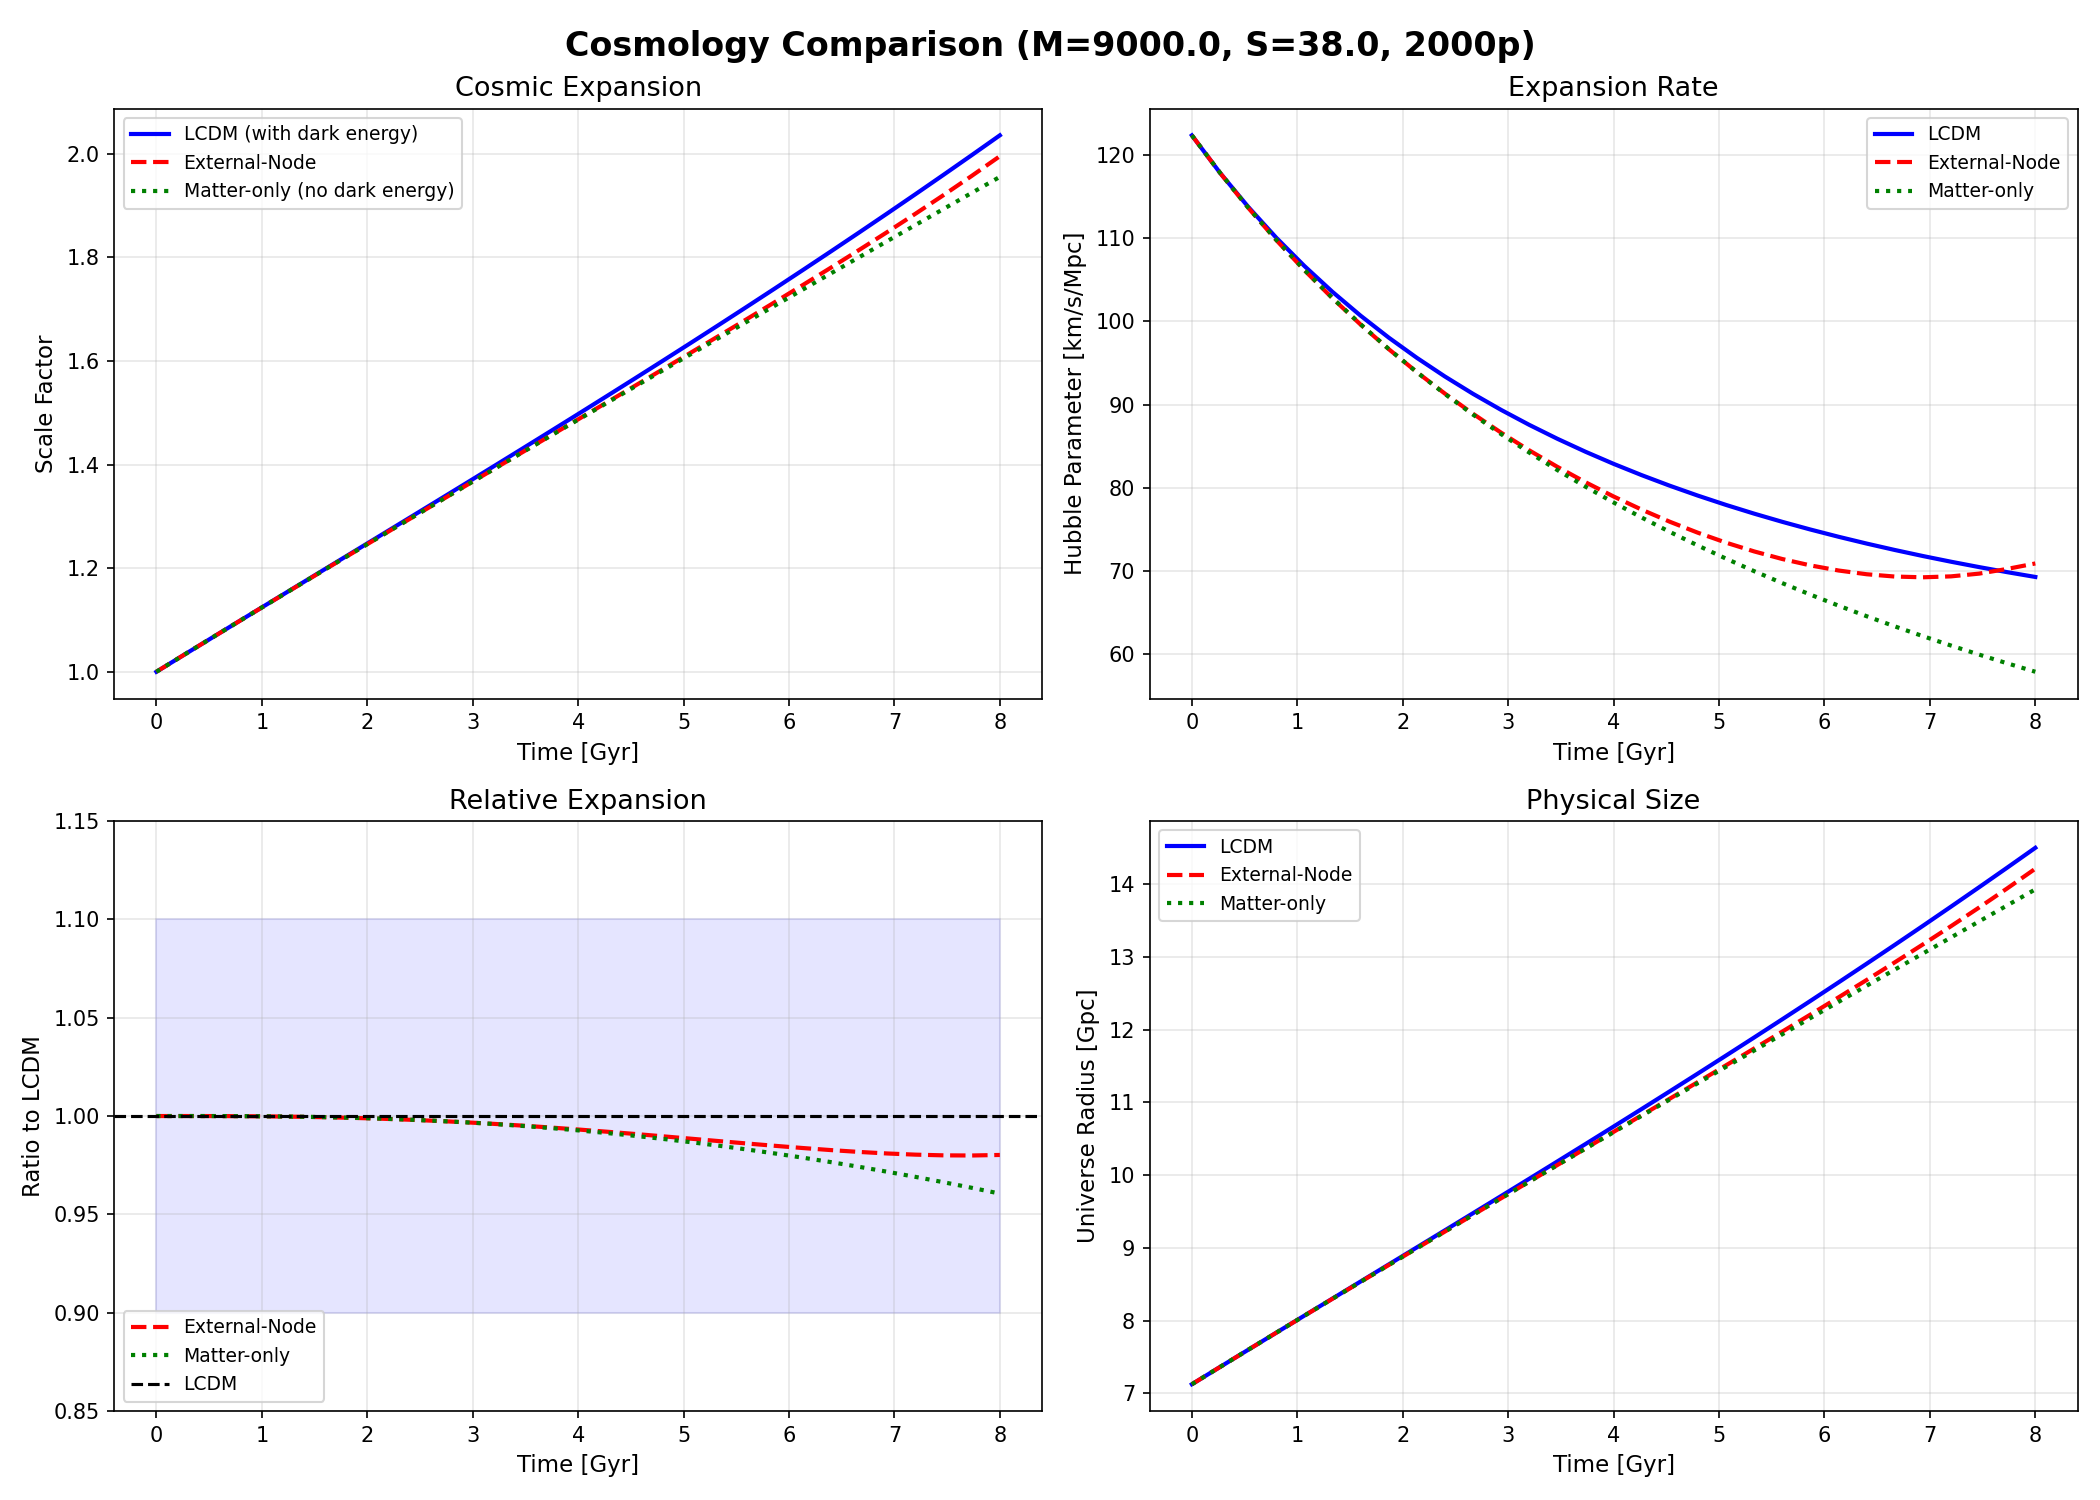
\includegraphics[width=1.0\linewidth]{fig3_4f97dec.png}
    \caption{$\Lambda$CDM (blue), External-Node M=9000$\times$M$_{obs}$, S=38 Gpc (red dashed), and matter-only (green dotted).
Top left: scale factor. Top right: Hubble parameter ($H_0 \approx 70$ km/s/Mpc). Bottom left: size ratio. Bottom right: universe size vs. node distance.
98.02\% endpoint match, $R^2 = 0.9954$ (size), $R^2 = 0.9630$ (expansion rate).}
\label{fig:primary}
\end{figure}

\begin{figure}[htbp]
    \centering
    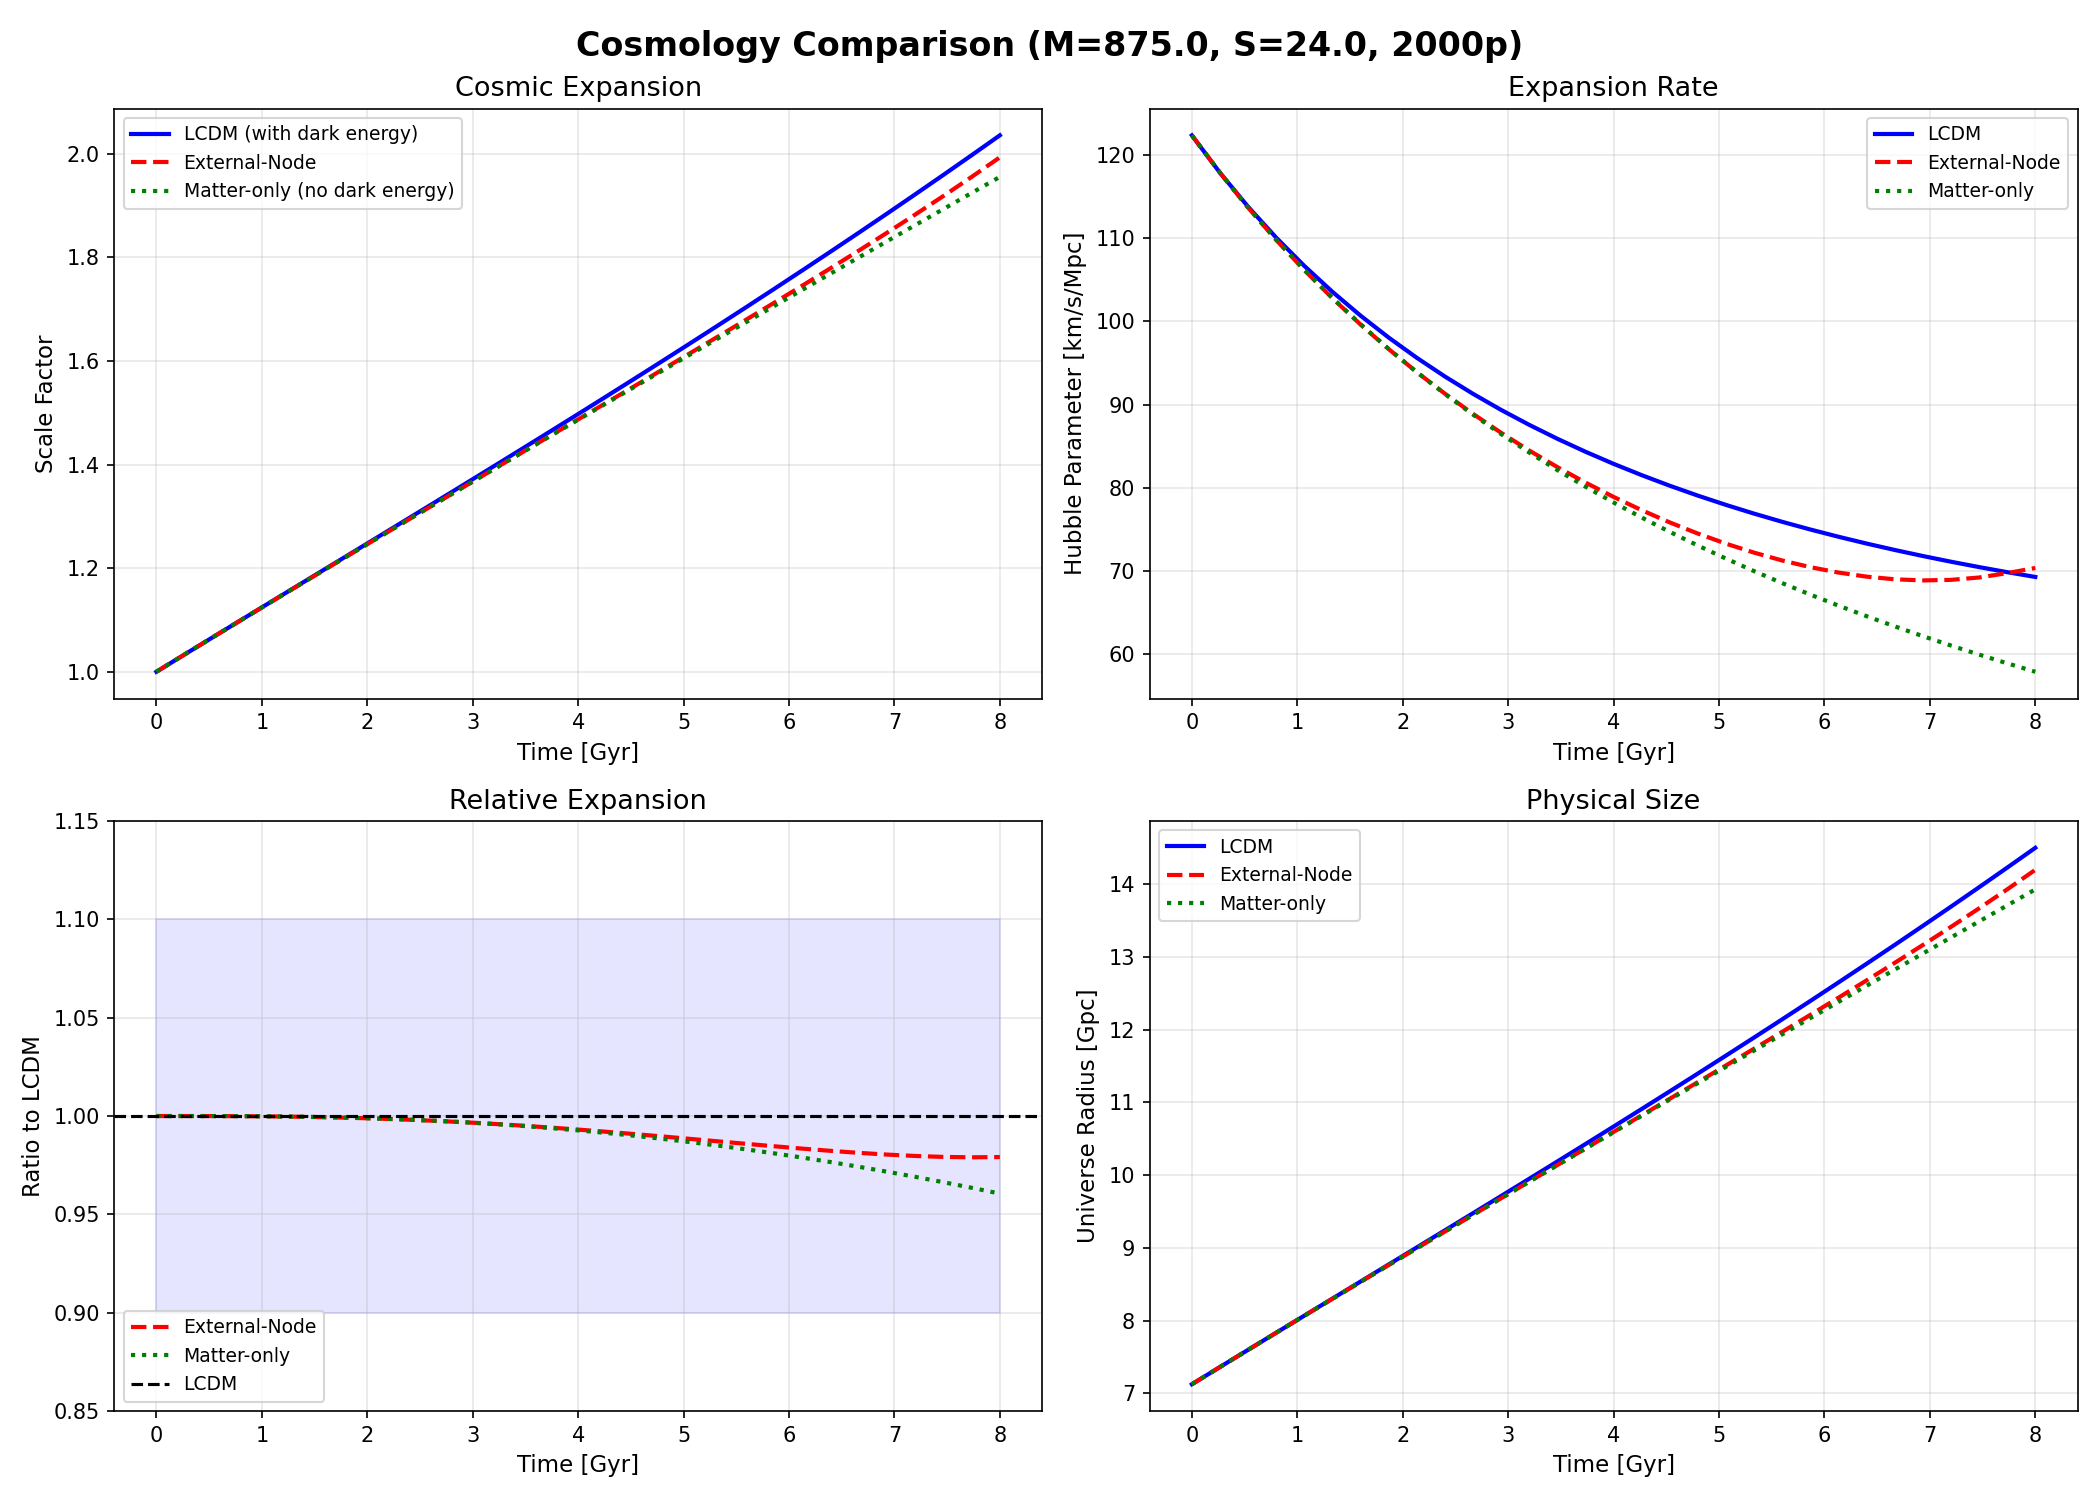
\includegraphics[width=0.87\linewidth]{fig2_4f97dec.png}
    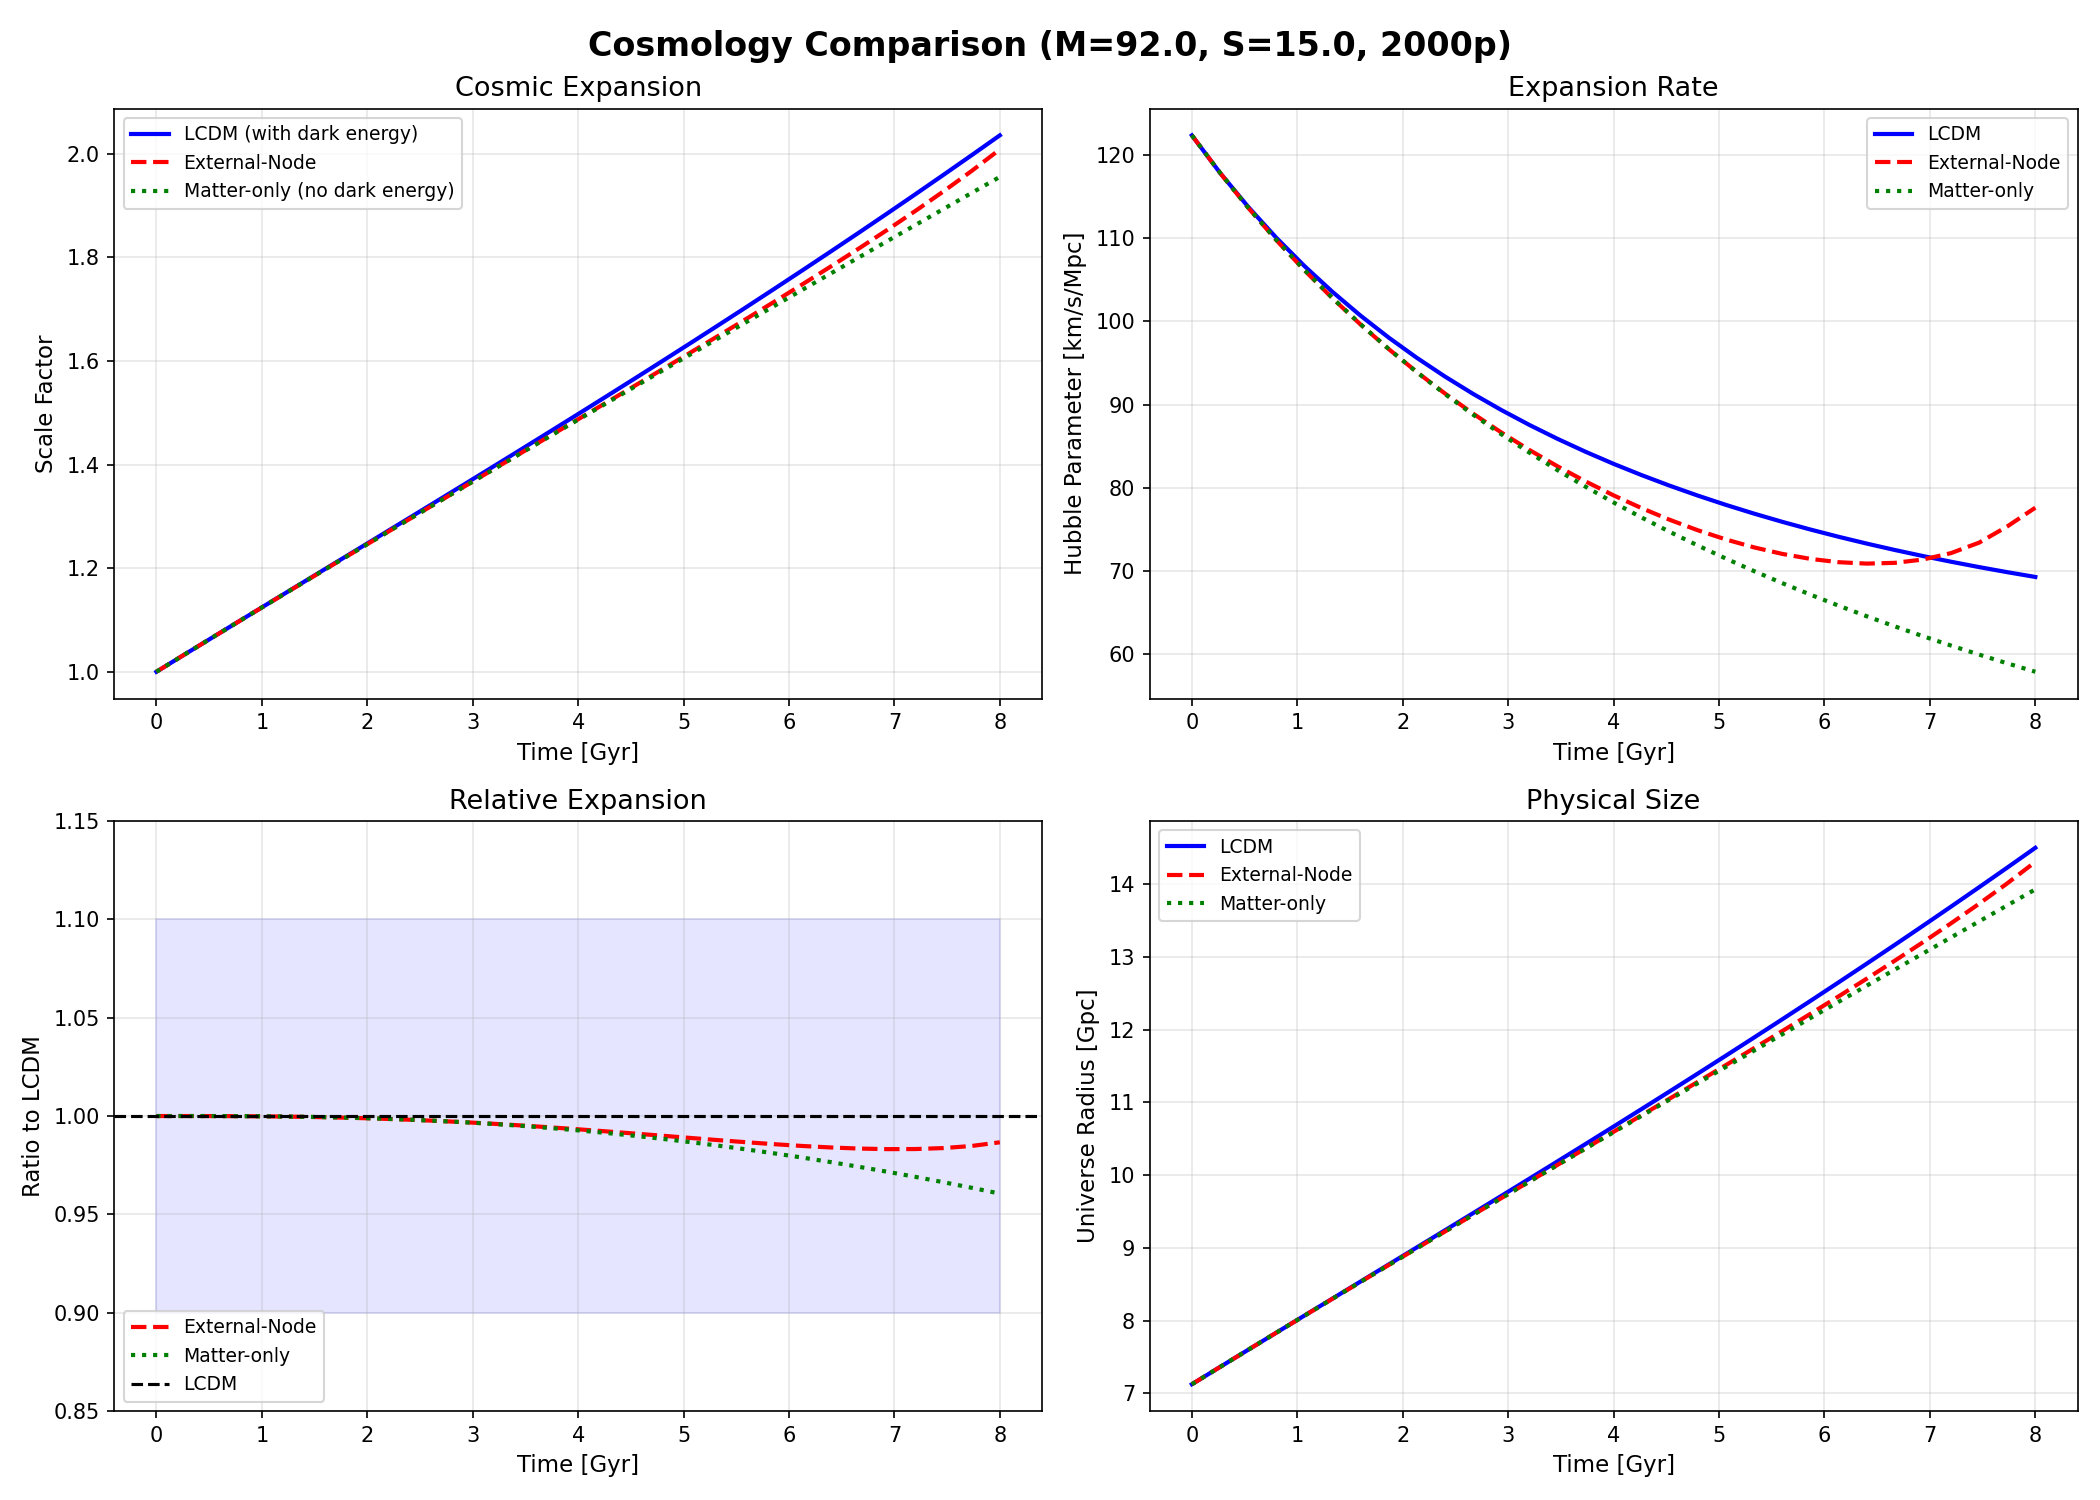
\includegraphics[width=0.87\linewidth]{fig1_4f97dec.png}
    \caption{Additional balanced-optimization configurations: (top) M=875$\times$M$_{obs}$, S=24 Gpc; (bottom) M=92$\times$M$_{obs}$, S=15 Gpc.
All achieve $R^2 > 0.99$ (size) and $R^2 > 0.95$ (expansion rate). Matter-only (green) consistently diverges.}
\label{fig:additional}
\end{figure}

\subsection{Parameter Space Exploration and Results}
\label{sec:results}

Multiple parameter combinations reproduce $\Lambda$CDM expansion (Table~\ref{tab:results}).
There is no unique optimal configuration. Rather, a family of solutions spans nearly two orders of magnitude in mass, as the tidal field depends on the ratio $M/S^3$; this scaling allows larger grid distances $S$ to compensate for larger nodal masses $M$, thereby alleviating the need for fine-tuning.

We use two optimization strategies:
\textbf{Balanced optimization} weights both size and expansion rate.
\textbf{Size-only optimization} maximizes size $R^2$ alone, at the cost of expansion rate (Section~\ref{sec:tradeoffs}).

\begin{table}[htbp]
\centering
\begin{tabular}{lcccc}
\toprule
\textbf{M} & \textbf{S [Gpc]} & \textbf{Endpoint} & \textbf{Size $R^2$} & \textbf{Expansion $R^2$} \\
\midrule
\multicolumn{5}{c}{\textit{Balanced optimization}} \\
$9000 \times M_{obs}$ & 38 & 98.02\% & 0.9954 & 0.9630 \\
$875 \times M_{obs}$ & 24 & 97.92\% & 0.9951 & 0.9603 \\
$92 \times M_{obs}$ & 15 & 98.67\% & 0.9966 & 0.9565 \\
\midrule
\multicolumn{5}{c}{\textit{Size-only optimization}} \\
$800 \times M_{obs}$ & 22 & 99.85\% & 0.9991 & (not optimized) \\
\midrule
\multicolumn{5}{c}{\textit{Baseline}} \\
Matter-only & --- & 96.06\% & 0.9890 & 0.8350 \\
\bottomrule
\end{tabular}
\caption{Parameter configurations and fit quality. Balanced optimization weights both size and expansion rate; size-only optimization maximizes size $R^2$ alone. Matter-only baseline uses no dark energy and no external nodes.}
\label{tab:results}
\end{table}

Smaller-$S$ configurations ($S = 15$ Gpc) may predict hyper-acceleration as the universe approaches the node boundary (Section~\ref{sec:phantom}).

\subsection{Optimization Tradeoffs: Model Accuracy and Expansion Dynamics}
\label{sec:tradeoffs}

Evaluating the model's performance requires balancing two distinct metrics: the fit to the cumulative expansion radius, $R(t)$, and the fit to the expansion rate, $H(t)$. Because the expansion rate is the first derivative of the radius, it imposes a more stringent constraint on the underlying dynamics. 

A ``size-only'' optimization can achieve a near-perfect fit to the final radius (e.g., $M=800 M_{obs}, S=22$ Gpc, $R^2_{size} = 0.9991$), yet fail to reproduce the correct expansion history, as the path integrates to the same displacement despite different local dynamics. By contrast, a balanced approach yields $R^2_{size} > 0.99$ and $R^2_{rate} > 0.95$, significantly outperforming the matter-only baseline ($R^2_{rate} \approx 0.84$). 

Two factors limit these rate comparisons. First, we compare our model's isotropic root-mean-square (RMS) expansion to the Friedmann $H(t)$, but the framework inherently predicts anisotropic expansion (Section~\ref{sec:dipole}); some discrepancy likely arises from this geometric effect. Second, the current Hubble tension ($\sim 8.6\%$) introduces inherent uncertainty into the ``target'' $H(t)$ of $\Lambda$CDM. 

\paragraph{Primary Results.}
Our primary configuration ($M_{ext} = 9000 M_{obs}$, $S = 38$ Gpc; Figure~\ref{fig:primary}) successfully tracks $\Lambda$CDM to within 2\% in total size ($R^2_{size} = 0.9954$) and matches the expansion history ($R^2_{rate} = 0.9630$), yielding an intrinsic $H_0 \approx 70$ km/s/Mpc without post-hoc adjustment.

\subsection{Matter-Only Comparison}
\label{sec:matter-only}

To demonstrate that our model generates true acceleration rather than a simple static fit, we compare it against a matter-only baseline (no dark energy and no external nodes). While the matter-only model can achieve a $\sim$96\% agreement in final universe size, the expansion rate $R^2$ reveals a significant divergence in the underlying physics (Table~\ref{tab:comparison}).


\begin{table}[htbp]
\centering
\begin{tabular}{lccc}
\toprule
\textbf{Model} & \textbf{Endpoint} & \textbf{Size $R^2$} & \textbf{Expansion $R^2$} \\
\midrule
$\Lambda$CDM (baseline) & 100\% & 1.0000 & 1.0000 \\
External-Node & 98.02\% & 0.9954 & 0.9630 \\
Matter-only & 96.06\% & 0.9890 & 0.8350 \\
\bottomrule
\end{tabular}
\caption{External-Node vs matter-only comparison for $M_{ext} = 9000 \times M_{obs}$, $S = 38$ Gpc. The expansion rate $R^2$ discriminates between genuine acceleration dynamics and coincidental endpoint agreement.}
\label{tab:comparison}
\end{table}

As shown in Table~\ref{tab:comparison}, the expansion rate $R^2$ serves as the definitive discriminator: our external-node model achieves a high $R^2$ of 0.96, whereas the matter-only model drops to 0.84. This discrepancy highlights that the matter-only approach produces a coincidental endpoint agreement by attempting to ``force'' a fit at a specific time, whereas the external-node model reproduces the genuine acceleration dynamics required to match the full expansion history.

\section{Scope and Limitations}
\label{sec:scope}
\label{sec:limitations}

This is a toy model, not a complete cosmological theory.
What it does not address:
\begin{itemize}
\item \textbf{General Relativity}: We use Newtonian gravity in flat Euclidean space. The tidal field is modeled as a pre-existing condition of the meta-structure, not as a force propagating from current node positions; nevertheless, a full GR treatment is needed to confirm the mechanism at these scales.
\item \textbf{Early Universe}: No treatment of inflation, baryogenesis, or nucleosynthesis. The Progenitor destabilization is posited, not derived.
\item \textbf{CMB Power Spectrum}: Effects on acoustic oscillations and Planck constraints are not computed \cite{Planck2020}.
\item \textbf{BAO}: Standard ruler constraints \cite{Eisenstein2005} have not been tested against this model.
\end{itemize}

\noindent A full theory would require relativistic treatment of the meta-structure's metric, tidal forces in curved spacetime, and a proper domain boundary for the Cosmological Principle.

We do not claim this model represents physical reality, but that classical alternatives to vacuum energy are viable and worth investigating.

\section{Predictions and Falsifiability}
\label{sec:predictions}
The model makes three distinct predictions, plus one qualitative consistency, all from the same lattice geometry.
Because the meta-structure is irregular (varying node masses and positions), it imprints angular signatures—dipole, quadrupole, octopole—sharing a common preferred direction.
Confirming or ruling out any one constrains the others.

\subsection{The Geometric ``Big Rip'' (Hyper-Acceleration)}
\label{sec:phantom}
$\Lambda$CDM predicts constant dark energy density and smooth exponential expansion ($w = -1$) forever.
The HMEA model predicts acceleration that strengthens over time.

\paragraph{Prediction:} As $R(t) \rightarrow S$, the tidal force scales as $(S-R)^{-2}$—acceleration increases as the universe approaches the nodes.

\paragraph{Observable:} The effective equation of state $w$ should drift below $-1$ (phantom energy \cite{Caldwell2003}), detectable via precision $w(z)$ measurements at low redshift.

\paragraph{Quantitative Analysis:}
The total effective equation of state $w_{eff} = -1 - \frac{2}{3}\frac{d \ln H}{d \ln a}$ characterizes the net expansion behavior.
For M=9000$\times$M$_{obs}$, S=38 Gpc, the current $R/S \approx 0.19$—well within the linear regime.
Phantom deviation grows as $R/S \rightarrow 1$.
Configurations with smaller $S$ (e.g., S=15 Gpc, $R/S \approx 0.48$) would show stronger present-day phantom signatures.

\subsection{Dipole Anisotropy}
\label{sec:dipole}
The Progenitor Hypothesis gives a roughly isotropic start, but the irregular meta-grid means the nearest HMEAs have different masses and distances.

\paragraph{Prediction:} Surveys (Euclid \cite{Euclid2011}, LSST \cite{LSST2019}) should detect a \textbf{dipole in the expansion rate}—one hemisphere expanding slightly faster than the other, toward the nearest or most massive HMEA.
This could contribute to the Hubble Tension: the $\sim$8.6\% discrepancy between CMB-calibrated ($\sim$67 km/s/Mpc) and distance-ladder ($\sim$73 km/s/Mpc) values of $H_0$ \cite{Riess2022, DiValentino2021}.
CMB-derived $H_0$ is an all-sky average; distance-ladder measurements sample specific directions.
A $\sim$5-11\% dipole could bias the latter relative to the former, producing an apparent method-dependent discrepancy.

\paragraph{Quantitative Estimate:}
Assuming 5\% position irregularity and 20\% mass variation (conservative for a virialized structure), with $\Omega_{\Lambda,eff} \equiv 2 G M_{ext} / (S^3 H_0^2)$, the tidal asymmetry propagates to $H_0$ via:

\[
\frac{\Delta H_0}{H_0} \approx \frac{1}{2} \cdot \frac{\Omega_{\Lambda,eff}}{\Omega_m + \Omega_{\Lambda,eff}} \cdot \sqrt{\left(\frac{2\delta_{eff}}{S - R}\right)^2 + \left(\frac{\Delta M_{eff}}{M}\right)^2}
\]

where $\delta_{eff} = \delta_{pos}/\sqrt{6}$ and $\Delta M_{eff} = \Delta M / \sqrt{6}$ account for statistical cancellation across 6 face nodes. Position and mass variations add in quadrature.
For M=9000$\times$M$_{obs}$, S=38 Gpc, $R \approx 7.25$ Gpc:

\begin{itemize}
    \item Position irregularity only (5\%): $\Delta H_0 / H_0 \approx 2.4\%$ (grid average)
    \item Mass variation only (20\%): $\Delta H_0 / H_0 \approx 3.9\%$ (grid average)
    \item \textbf{Combined (position + mass)}: $\Delta H_0 / H_0 \approx 4.6\%$ ($\sim$3.2 km/s/Mpc, grid average)
    \item \textbf{Single nearest node (worst case)}: $\Delta H_0 / H_0 \approx 11.3\%$ ($\sim$7.9 km/s/Mpc)
    \item Observed Hubble Tension: $\sim$8.6\% (6 km/s/Mpc difference between 67 and 73 km/s/Mpc)
\end{itemize}

\paragraph{Implications:}
The predicted dipole ($\sim$4.6\% grid average, up to $\sim$11.3\% worst case) brackets the Hubble Tension ($\sim$8.6\%).
Detection of a $\sim$5-11\% $H_0$ dipole uncorrelated with local structure would support the model; absence of any dipole above $\sim$2\% would constrain it.

\subsection{CMB Large-Angle Anomalies (The ``Axis of Evil'')}
\label{sec:axis-of-evil}

The CMB quadrupole ($l=2$) and octopole ($l=3$) share a preferred axis at a level inconsistent with isotropy ($p < 0.5\%$) \cite{Land2005, deOliveiraCosta2004, Copi2006}.
$\Lambda$CDM offers no explanation.

\paragraph{Prediction:}
The HMEA lattice has nodes at three distinct distances: 6 face nodes at $S$, 12 edge at $S\sqrt{2}$, 8 corner at $S\sqrt{3}$.
This discrete geometry imprints angular modes on the tidal field:
\begin{itemize}
    \item \textbf{Dipole} ($l=1$): nearest node closer or more massive than opposing node (Section~\ref{sec:dipole}).
    \item \textbf{Quadrupole} ($l=2$): face-node asymmetries along the three principal axes.
    \item \textbf{Octopole} ($l=3$): corner-node tetrahedral sub-symmetry.
\end{itemize}

All multipoles come from the same lattice, so their axes are necessarily correlated—matching the observed alignment.
The Progenitor Hypothesis reinforces this: expanding matter inherits the tidal imprint from the start.
The correlation with the ecliptic plane is likely coincidental.

\paragraph{Qualitative Comparison:}
Observed anomalies \cite{Copi2010}: (1) low quadrupole power, (2) planar octopole, (3) $l=2$/$l=3$ alignment.
The model accounts for all three: cubic symmetry partially cancels the quadrupole, corner nodes project onto lattice planes, and both modes share the same structure.

\paragraph{Test:}
The predicted $H_0$ dipole should be \textbf{aligned with the Axis of Evil} ($l \approx 260°$, $b \approx 60°$).
A dipole orthogonal to it would disfavor a single-lattice origin.

\subsection{Dark Flow and Large-Scale Bulk Motions}
\label{sec:dark-flow}

Lattice asymmetry produces a net acceleration on the entire bubble—not just a differential expansion rate, but a coherent bulk motion.
Unlike local peculiar velocities (which average out at large scales), this externally-sourced flow is scale-independent.

Watkins et al. \cite{Watkins2023} measured a bulk flow of $419 \pm 36$ km/s at $\sim$290 Mpc using CosmicFlows-4—4.8$\sigma$ tension with $\Lambda$CDM.
Follow-up analysis \cite{Watkins2025} showed this flow is dominated by \textbf{sources external to the survey volume}—exactly what trans-observable structure predicts.
Dark flow ($l \approx 290$-$298°$), the Axis of Evil ($l \approx 260°$), and the CMB dipole all point to the same general sky region—expected if all trace the nearest HMEA.

The HMEA model naturally produces such flows, but we do not attempt a quantitative estimate here: the predicted bulk velocity depends on the same irregularity parameters used in the dipole estimate (Section~\ref{sec:dipole}), so it would not constitute an independent test.

\section{Observational Consistency: The ``Dark Giant'' Principle}
\label{sec:defenses}
Why don't we see objects of $\sim 10^{55}$ kg?
HMEAs are most plausibly ancient black holes ($t_{node} \gg 13.8$ Gyr) that cleared their local fuel supply long ago.
Without an accretion disk, a black hole is electromagnetically silent.
Hawking radiation is negligible: $T_H \propto 1/M$ gives $T_H \sim 10^{-83}$ K at these masses.

\section{The ``Great Metabolism'' Hypothesis}
\label{sec:metabolism}
\textit{(Speculative---not derived from simulation results.)}

The HMEA framework suggests a cyclical cosmology:
\begin{enumerate}
\item \textbf{Expansion}: A node destabilizes (Big Bang), filling a void with matter—effectively a macroscopic accretion disk transporting mass across the void.
\item \textbf{Feeding}: Galaxies are stripped and accreted onto neighboring HMEAs.
\item \textbf{Destabilization}: An HMEA accumulates critical mass or merges with a neighbor.
\item \textbf{Re-Ignition}: The node detonates, initiating a new cycle.
\end{enumerate}

Our universe is a transient structure: a pulse of matter facilitating mass transfer between nodes in an eternal lattice.

\section{Conclusion}
\label{sec:conclusion}
The External-Node Model replaces dark energy with tidal gravity from trans-observable structure.
N-body simulations show that configurations spanning M=92-9000$\times$M$_{obs}$, S=15-38 Gpc reproduce $\Lambda$CDM expansion with $R^2 > 0.95$ (expansion rate) and $R^2 > 0.99$ (size) over 8 Gyr, using only classical physics.

The same geometry produces patterns consistent with three anomalies usually treated as unrelated: the Hubble Tension ($\Delta H_0/H_0 \approx 5$-$11\%$), the CMB Axis of Evil, and dark flow.
In this model, all three are consequences of a single geometric structure.

Future work: full GR formulation, systematic parameter constraints analogous to $\Omega_\Lambda$ fitting from SNe~Ia data, quantitative CMB multipole predictions from the lattice, and directional coherence tests using Euclid and LSST data.
If the predicted alignment between the $H_0$ dipole, CMB multipoles, and bulk flow is confirmed, dark energy may not be an intrinsic property of spacetime, but a consequence of our position within a larger gravitational structure.

\begin{thebibliography}{99}
\bibitem{Planck2020} Planck Collaboration. "Planck 2018 results. VI. Cosmological parameters." \textit{Astronomy \& Astrophysics} 641, A6 (2020).
\bibitem{Weinberg1989} Weinberg, S. "The cosmological constant problem." \textit{Reviews of Modern Physics} 61.1: 1 (1989).
\bibitem{Steinhardt1999} Zlatev, I., Wang, L., and Steinhardt, P. J. "Quintessence, cosmic coincidence, and the cosmological constant." \textit{Physical Review Letters} 82.5: 896 (1999).
\bibitem{Riess2022} Riess, A. G., et al. "A Comprehensive Measurement of the Local Value of the Hubble Constant with 1 km/s/Mpc Uncertainty." \textit{The Astrophysical Journal Letters} 934.1: L7 (2022).
\bibitem{Land2005} Land, K. and Magueijo, J. "Examination of evidence for a preferred axis in the cosmic radiation anisotropy." \textit{Physical Review Letters} 95.7: 071301 (2005).
\bibitem{Watkins2023} Watkins, R., et al. "Analysing the large-scale bulk flow using CosmicFlows4." \textit{Monthly Notices of the Royal Astronomical Society} 524.2: 1885 (2023).
\bibitem{Riess1998} Riess, A. G., et al. "Observational evidence from supernovae for an accelerating universe and a cosmological constant." \textit{The Astronomical Journal} 116.3: 1009 (1998).
\bibitem{Perlmutter1999} Perlmutter, S., et al. "Measurements of $\Omega$ and $\Lambda$ from 42 high-redshift supernovae." \textit{The Astrophysical Journal} 517.2: 565 (1999).
\bibitem{MersiniHoughton2009} Mersini-Houghton, L. and Holman, R. "``Tilting'' the universe with the landscape multiverse: the dark flow." \textit{Journal of Cosmology and Astroparticle Physics} 2009.02: 006 (2009).
\bibitem{Kashlinsky2008} Kashlinsky, A., et al. "A measurement of large-scale peculiar velocities of clusters of galaxies: results and cosmological implications." \textit{The Astrophysical Journal} 686.2: L49 (2008).
\bibitem{Eisenstein2005} Eisenstein, D. J., et al. "Detection of the baryon acoustic peak in the large-scale correlation function of SDSS luminous red galaxies." \textit{The Astrophysical Journal} 633.2: 560 (2005).
\bibitem{Caldwell2003} Caldwell, R. R., Kamionkowski, M., and Weinberg, N. N. "Phantom energy and cosmic doomsday." \textit{Physical Review Letters} 91.7: 071301 (2003).
\bibitem{Euclid2011} Laureijs, R., et al. "Euclid Definition Study Report." arXiv preprint arXiv:1110.3193 (2011).
\bibitem{LSST2019} Ivezić, Ž., et al. "LSST: from science drivers to reference design and anticipated data products." \textit{The Astrophysical Journal} 873.2: 111 (2019).
\bibitem{DiValentino2021} Di Valentino, E., et al. "In the realm of the Hubble tension—a review of solutions." \textit{Classical and Quantum Gravity} 38.15: 153001 (2021).
\bibitem{deOliveiraCosta2004} de Oliveira-Costa, A., et al. "Significance of the largest scale CMB fluctuations in WMAP." \textit{Physical Review D} 69.6: 063516 (2004).
\bibitem{Copi2006} Copi, C. J., et al. "On the large-angle anomalies of the microwave sky." \textit{Monthly Notices of the Royal Astronomical Society} 367.1: 79-102 (2006).
\bibitem{Copi2010} Copi, C. J., et al. "Large-angle anomalies in the CMB." \textit{Advances in Astronomy} 2010: 847541 (2010).
\bibitem{Watkins2025} Watkins, R. and Feldman, H. A. "The bulk flow of galaxy surveys." arXiv preprint arXiv:2512.03168 (2025).
\end{thebibliography}
\end{document}